\documentclass[aspectratio=43]{beamer}

% Title --------------------------------------------
\title{\huge Long-term legacies of wars}
\author{Francisco Villamil}
\date{War, peace, and political violence\\UC3M, Fall 2023}

%%% NOTE -- CHECK THIS: https://github.com/paulgp/beamer-tips


%%% Building heavily on https://github.com/kylebutts/templates

% xcolor, define them
\usepackage{xcolor}

% TEXT COLORS
\definecolor{red}{HTML}{9a2515}
\definecolor{yellow}{HTML}{EBC944}
\definecolor{asher}{HTML}{555F61}
\definecolor{jet}{HTML}{131516}

% THEME COLORS
\definecolor{accent}{HTML}{107895}
\definecolor{accent2}{HTML}{9a2515}

% Color commands
\newcommand\red[1]{{\color{red}#1}}
\newcommand\yellow[1]{{\color{yellow}#1}}
\newcommand\asher[1]{{\color{asher}#1}}

\newcommand\BGred[1]{{\colorbox{red!80!white}{#1}}}
\newcommand\BGyellow[1]{{\colorbox{yellow!80!white}{#1}}}
\newcommand\BGasher[1]{{\colorbox{asher!80!white}{#1}}}

\renewcommand<>{\BGyellow}[1]{\only#2{\beameroriginal{\BGyellow}}{#1}}

% Appendix numbering
\usepackage{appendixnumberbeamer}

% Beamer Options -------------------------------------

% Background
\setbeamercolor{background canvas}{bg = white}

% Change text margins
\setbeamersize{text margin left = 25pt, text margin right = 15pt}

% \alert
\setbeamercolor{alerted text}{fg = accent2}

% Frame title
\setbeamercolor{frametitle}{bg = white, fg = jet}
\setbeamercolor{framesubtitle}{bg = white, fg = accent}
\setbeamerfont{framesubtitle}{size = \small, shape = \itshape}

% Block
\setbeamercolor{block title}{fg = white, bg = accent2}
\setbeamercolor{block body}{fg = jet, bg = jet!10!white}

% Title page
\setbeamercolor{title}{fg = jet}
\setbeamercolor{subtitle}{fg = accent}

%% Custom \maketitle and \titlepage
\setbeamertemplate{title page}
{
    \begin{centering}
      % \vspace{20mm}
      {\Large \usebeamerfont{title}\usebeamercolor[fg]{title}\inserttitle}\\ \vskip0.25em%
      \ifx\insertsubtitle\@empty%
      \else%
        {\usebeamerfont{subtitle}\usebeamercolor[fg]{subtitle}\insertsubtitle\par}%
      \fi%
      {\vspace{10mm}\insertauthor}\\
      \ifx\insertinstitute\@empty%
      \else%
        {\vspace{5mm}\color{asher}\scriptsize{\insertinstitute}}
      \fi%
      {\color{asher}\small{\insertdate}}\\
    \end{centering}
}

% Table of Contents
\setbeamercolor{section in toc}{fg = accent!70!jet}
\setbeamercolor{subsection in toc}{fg = jet}

% Button
\setbeamercolor{button}{bg = accent}

% Remove navigation symbols
\setbeamertemplate{navigation symbols}{}

% Table and Figure captions
\setbeamercolor{caption}{fg=jet!70!white}
\setbeamercolor{caption name}{fg=jet}
\setbeamerfont{caption name}{shape = \itshape}

% Put slide number / total slides at the bottom right
\makeatother
\makeatletter
\setbeamertemplate{footline} %{\hfill\insertframenumber/\inserttotalframenumber}
{%
  \leavevmode%
  \hbox{
  \begin{beamercolorbox}[wd=\paperwidth,ht=2.5ex,dp=1.125ex,leftskip=.3cm,rightskip=.3cm plus1fil]{footlinecolor}%
    \color{asher}{\hfill\insertframenumber/\inserttotalframenumber}
  \end{beamercolorbox}}%
  \vskip0pt%
}
\makeatother
\makeatletter

% Bullet points

%% Fix left-margins
\settowidth{\leftmargini}{\usebeamertemplate{itemize item}}
\addtolength{\leftmargini}{\labelsep}

%% enumerate item color
\setbeamercolor{enumerate item}{fg = accent}
\setbeamerfont{enumerate item}{size = \small}
\setbeamertemplate{enumerate item}{\insertenumlabel.}

%% itemize
\setbeamercolor{itemize item}{fg = accent!70!white}
\setbeamerfont{itemize item}{size = \small}
\setbeamertemplate{itemize item}[circle]
\setlength{\itemsep}{0pt plus 6pt}

%% right arrow for subitems
\setbeamercolor{itemize subitem}{fg = accent!60!white}
\setbeamerfont{itemize subitem}{size = \small}
\setbeamertemplate{itemize subitem}{$\rightarrow$}

\setbeamertemplate{itemize subsubitem}[square]
\setbeamercolor{itemize subsubitem}{fg = jet}
\setbeamerfont{itemize subsubitem}{size = \small}

% References

%% Bibliography Font, roughly matching aea
\setbeamerfont{bibliography item}{size = \footnotesize}
\setbeamerfont{bibliography entry author}{size = \footnotesize, series = \bfseries}
\setbeamerfont{bibliography entry title}{size = \footnotesize}
\setbeamerfont{bibliography entry location}{size = \footnotesize, shape = \itshape}
\setbeamerfont{bibliography entry note}{size = \footnotesize}

\setbeamercolor{bibliography item}{fg = jet}
\setbeamercolor{bibliography entry author}{fg = accent!60!jet}
\setbeamercolor{bibliography entry title}{fg = jet}
\setbeamercolor{bibliography entry location}{fg = jet}
\setbeamercolor{bibliography entry note}{fg = jet}

%% Remove bibliography symbol in slides
\setbeamertemplate{bibliography item}{}





% Links ----------------------------------------------

\usepackage{hyperref}
\hypersetup{
  colorlinks = true,
  linkcolor = accent,
  filecolor = accent,
  urlcolor = accent,
  citecolor = accent,
}


% Line spacing --------------------------------------
\usepackage{setspace}
\setstretch{1.2}


% \begin{columns} -----------------------------------
\usepackage{multicol}


% % Fonts ---------------------------------------------
% % Beamer Option to use custom fonts
% \usefonttheme{professionalfonts}
%
% % \usepackage[utopia, smallerops, varg]{newtxmath}
% % \usepackage{utopia}
% \usepackage[sfdefault,light]{roboto}
%
% % Small adjustments to text kerning
% \usepackage{microtype}



% Remove annoying over-full box warnings -----------
\vfuzz2pt
\hfuzz2pt


% Table of Contents with Sections
\setbeamerfont{myTOC}{series=\bfseries, size=\Large}
\AtBeginSection[]{
        \frame{
            \frametitle{Roadmap}
            \tableofcontents[current]
        }
    }


% References ----------------------------------------
\usepackage[
    citestyle= authoryear,
    style = authoryear,
    natbib = true,
    backend = biber
]{biblatex}

% Smaller font-size for references
\renewcommand*{\bibfont}{\small}

% Remove "In:"
\renewbibmacro{in:}{}

% Color citations for slides
\newenvironment{citecolor}
    {\footnotesize\begin{color}{accent2}}
    {\end{color}}

\newcommand{\citetcolor}[1]{{\footnotesize\textcolor{asher}{\citet{#1}}}}
\newcommand{\citepcolor}[1]{{\footnotesize\textcolor{asher}{\citep{#1}}}}

% Tables -------------------------------------------
% Tables too big
% \begin{adjustbox}{width = 1.2\textwidth, center}
\usepackage{adjustbox}
\usepackage{array}
\usepackage{threeparttable, booktabs, adjustbox}

% Fix \input with tables
% \input fails when \\ is at end of external .tex file

\makeatletter
\let\input\@@input
\makeatother

% Tables too narrow
% \begin{tabularx}{\linewidth}{cols}
% col-types: X - center, L - left, R -right
% Relative scale: >{\hsize=.8\hsize}X/L/R
\usepackage{tabularx}
\newcolumntype{L}{>{\raggedright\arraybackslash}X}
\newcolumntype{R}{>{\raggedleft\arraybackslash}X}
\newcolumntype{C}{>{\centering\arraybackslash}X}

% Figures

% \imageframe{img_name} -----------------------------
% from https://github.com/mattjetwell/cousteau
\newcommand{\imageframe}[1]{%
    \begin{frame}[plain]
        \begin{tikzpicture}[remember picture, overlay]
            \node[at = (current page.center), xshift = 0cm] (cover) {%
                \includegraphics[keepaspectratio, width=\paperwidth, height=\paperheight]{#1}
            };
        \end{tikzpicture}
    \end{frame}%
}

% subfigures
\usepackage{subfigure}


% Highlight slide -----------------------------------
% \begin{transitionframe} Text \end{transitionframe}
% from paulgp's beamer tips
\newenvironment{transitionframe}{
    \setbeamercolor{background canvas}{bg=accent!60!black}
    \begin{frame}\color{accent!10!white}\LARGE\centering
}{
    \end{frame}
}


% Table Highlighting --------------------------------
% Create top-left and bottom-right markets in tabular cells with a unique matching id and these commands will outline those cells
\usepackage[beamer,customcolors]{hf-tikz}
\usetikzlibrary{calc}
\usetikzlibrary{fit,shapes.misc}

% To set the hypothesis highlighting boxes red.
\newcommand\marktopleft[1]{%
    \tikz[overlay,remember picture]
        \node (marker-#1-a) at (0,1.5ex) {};%
}
\newcommand\markbottomright[1]{%
    \tikz[overlay,remember picture]
        \node (marker-#1-b) at (0,0) {};%
    \tikz[accent!80!jet, ultra thick, overlay, remember picture, inner sep=4pt]
        \node[draw, rectangle, fit=(marker-#1-a.center) (marker-#1-b.center)] {};%
}



\begin{document}

\begin{frame}
  \titlepage
\end{frame}

% ----------------------------------------------------
\imageframe{img/sant_felip_neri}
% ----------------------------------------------------

% ----------------------------------------------------
\begin{frame}
\frametitle{The consequences of wars}
\centering

\begin{itemize}
  \item Economic
  \item<2-> Social and institutional
  \item<3-> Social processes of war
  \item<4-> Legacies of violence
  \item<5->[]
  \item<5-> {\color{red}{\textbf{Differences} between interstate and civil wars?}}
\end{itemize}

\end{frame}
% ----------------------------------------------------

% ----------------------------------------------------
\begin{frame}
\frametitle{Economic consequences}
\centering

\begin{itemize}[<+->]
  \item War explains growth collapse in developing countries since the 70s
  \item It's difficult to measure it
  \begin{itemize}
    \item Reverse causality: same problem with the effect of economic growth on conflict
    \item What if a bad economic situation is the continuation of pre-war trends?
  \end{itemize}
  \item The question is {\color{red}{\textbf{how}}} it affects the economy, e.g.
  \begin{itemize}
    \item Different conflicts, different effects?
    \item How long its legacies last? How?
  \end{itemize}
\end{itemize}

\end{frame}
% ----------------------------------------------------

% ----------------------------------------------------
\imageframe{img/Apocalypse_vasnetsov}
% ----------------------------------------------------

% ----------------------------------------------------
\imageframe{img/black_death}
% ----------------------------------------------------


% ----------------------------------------------------
\begin{frame}
\frametitle{Economic consequences of war}
\centering

\begin{minipage}{0.59\textwidth}\centering
\begin{itemize}
  \item<2-> Main argument: inequality only decreases after mass violence or catastrophes
  \item<3-> The \red{`Four Horsemen'} of leveling: mass-mobilization warfare, transformative revolutions, state collapse, and catastrophic plagues
  \item<4-> Situations when the rich have more to lose and/or the poor increase their relative power
\end{itemize}
\end{minipage}\hfill
\begin{minipage}{0.39\textwidth}\centering
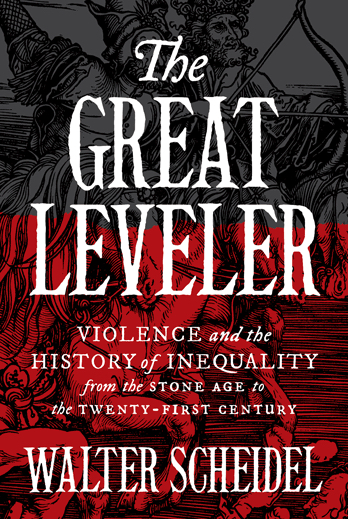
\includegraphics[width = \textwidth]{img/scheidel}\\\vspace{10pt}
{\small Walter Scheidel (2018)}
\end{minipage}

\end{frame}
% ----------------------------------------------------

% % ----------------------------------------------------
% \begin{frame}
% \frametitle{Economic consequences}
% \centering
%
% \begin{minipage}{0.39\textwidth}\centering
% \begin{itemize}
%   \only<1>{\item Int'l wars that involve \red{mass-mobilization} decrease inequality
%   \item Different to old wars
%   \item[] {\small (winers win, losers lose, inequality increases)}}
%   \only<2>{\item What about \BGyellow{civil wars}? Similar to pre-modern wars, inequality increases: increased value of capital, war confiscations, etc
%   \begin{itemize}
%     \item Civil war $\neq$ revolution, but often go together
%   \end{itemize}}
% \end{itemize}
% \end{minipage}\hfill
% \begin{minipage}{0.59\textwidth}\centering
% 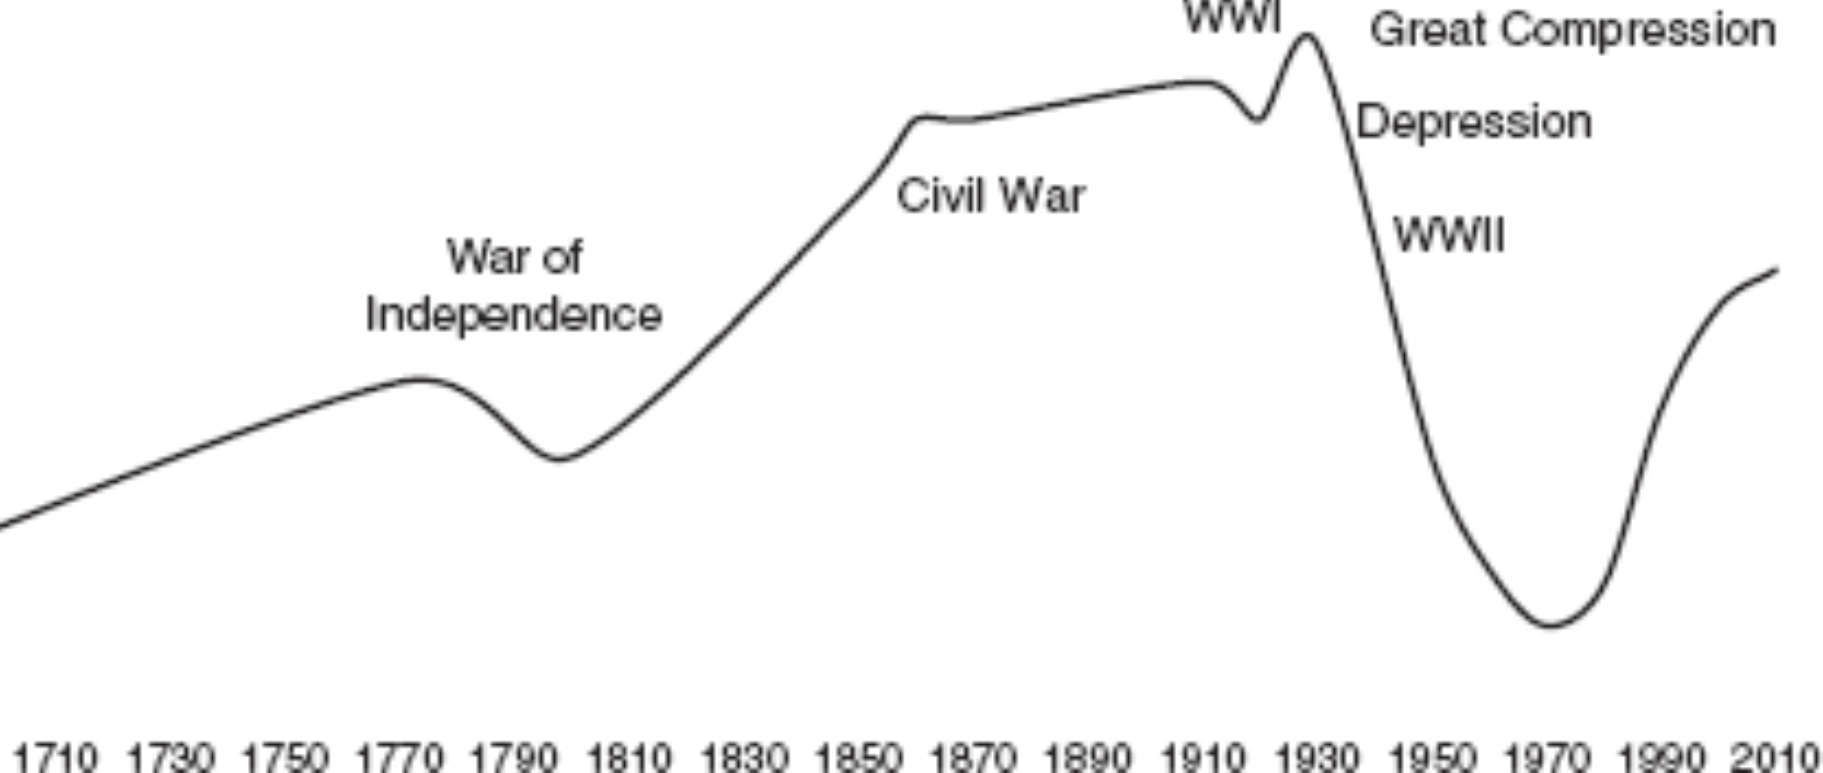
\includegraphics[width = \textwidth]{img/ineq-us}\\\vspace{5pt}
% {\footnotesize Inequality in the US (Scheidel 2018)}\\\vspace{15pt}
% 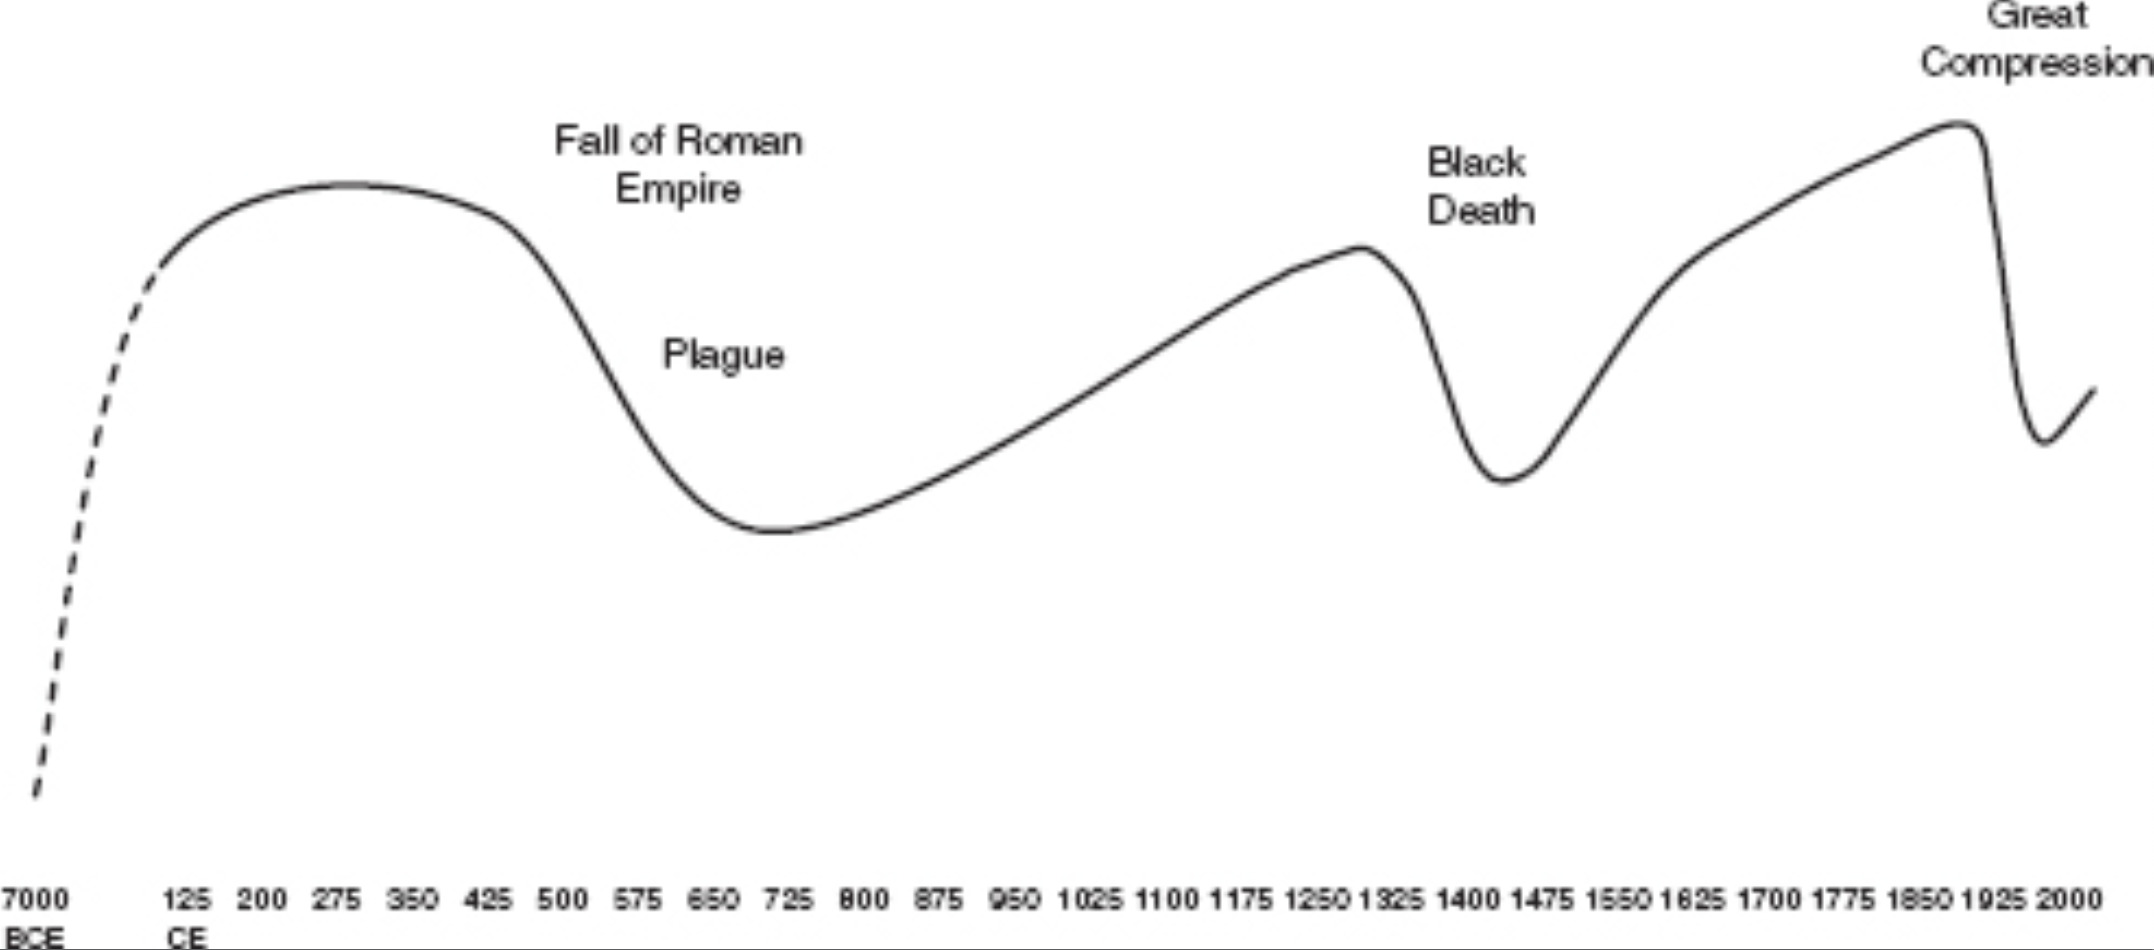
\includegraphics[width = \textwidth]{img/ineq-long-term-europe}\\\vspace{5pt}
% {\footnotesize Long-term trend in Europe}
% \end{minipage}
%
% \end{frame}
% % ----------------------------------------------------

% ----------------------------------------------------
\begin{frame}
\frametitle{Scheidel's \textit{The great leveler}}
\centering

\begin{itemize}
  \item Inter-state wars that involve {\color{red}{mass-mobilization}} decrease inequality
  \item Different to pre-modern wars {\small (winers win, losers lose, more inequality)}
  \item<2-> {\color{red}{What about civil wars?}} Similar to pre-modern wars, inequality increases: increased value of capital, war confiscations, etc
  \begin{itemize}
    \item Civil war $\neq$ revolution, but often go together
  \end{itemize}
\end{itemize}


\end{frame}
% ----------------------------------------------------

% ----------------------------------------------------
\begin{frame}
\frametitle{Inequality over time}
\centering

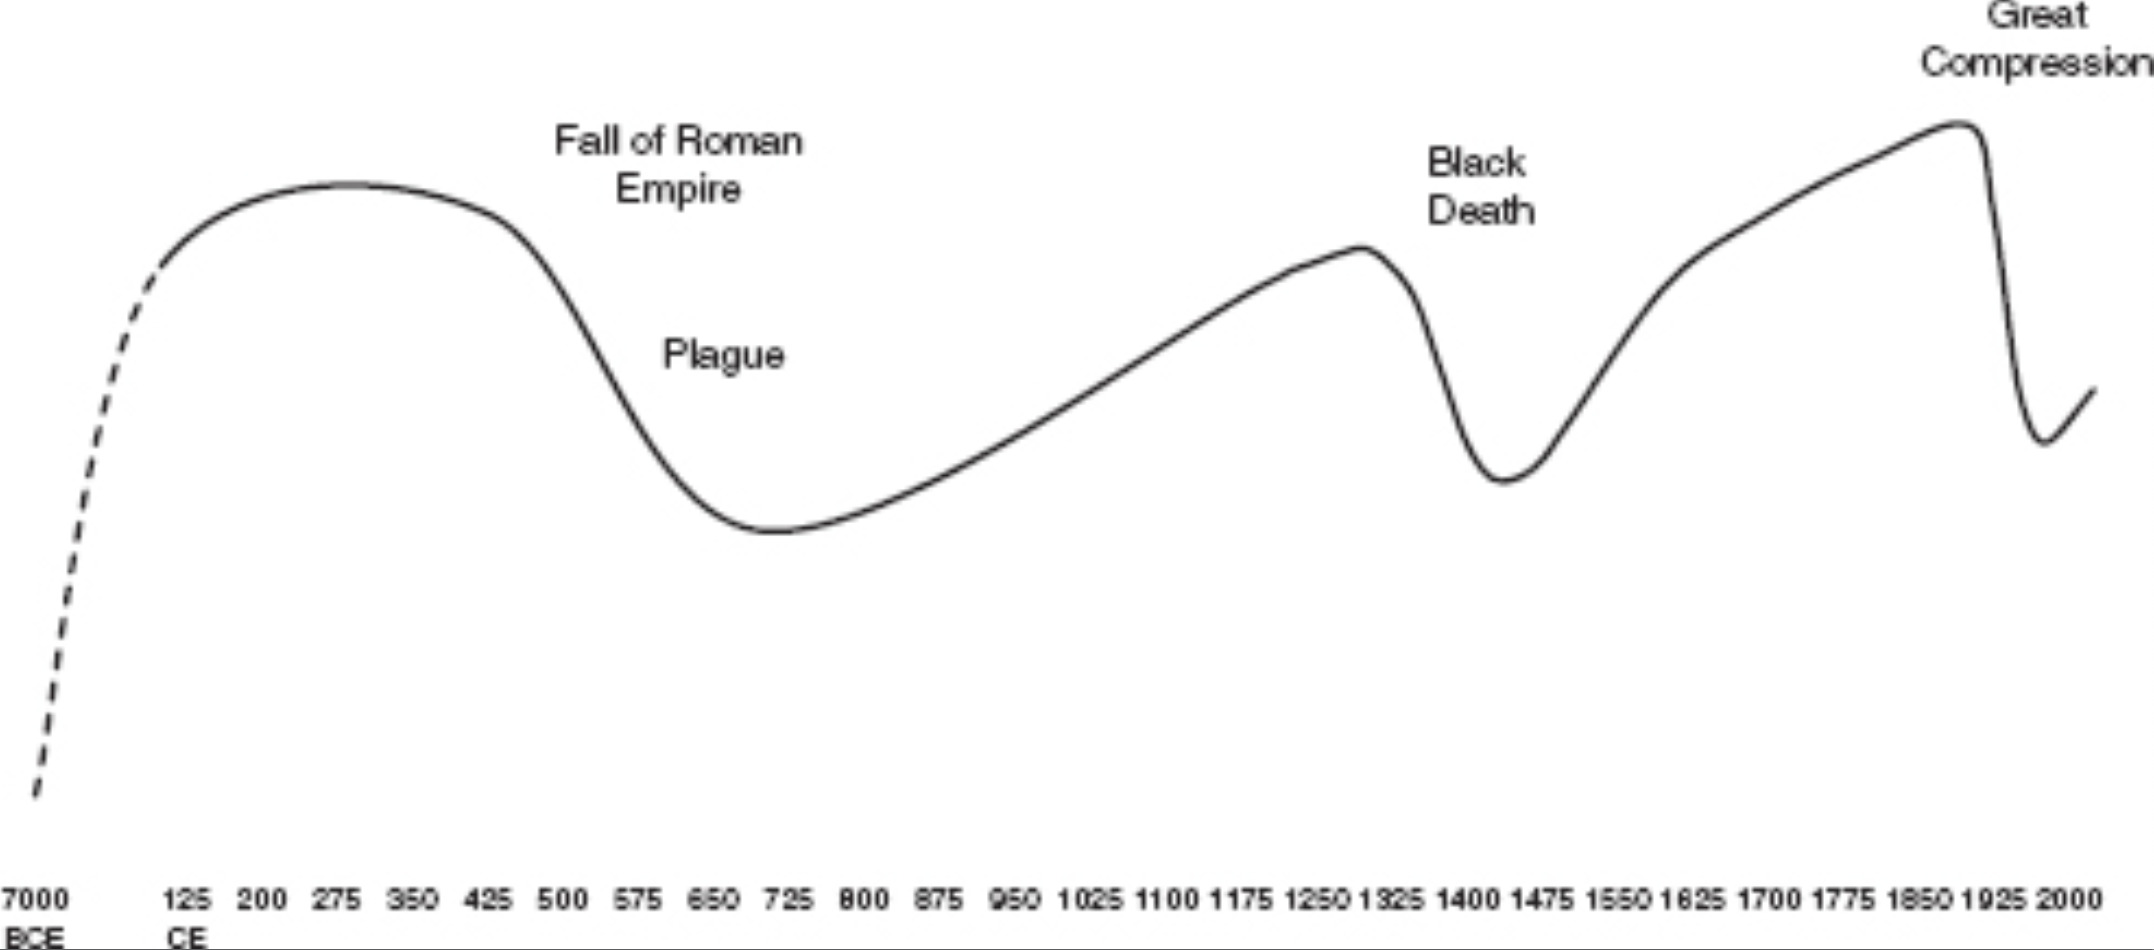
\includegraphics[width = \textwidth]{img/ineq-long-term-europe}\\\vspace{15pt}Europe

\end{frame}
% ----------------------------------------------------

% ----------------------------------------------------
\begin{frame}
\frametitle{Inequality over time}
\centering

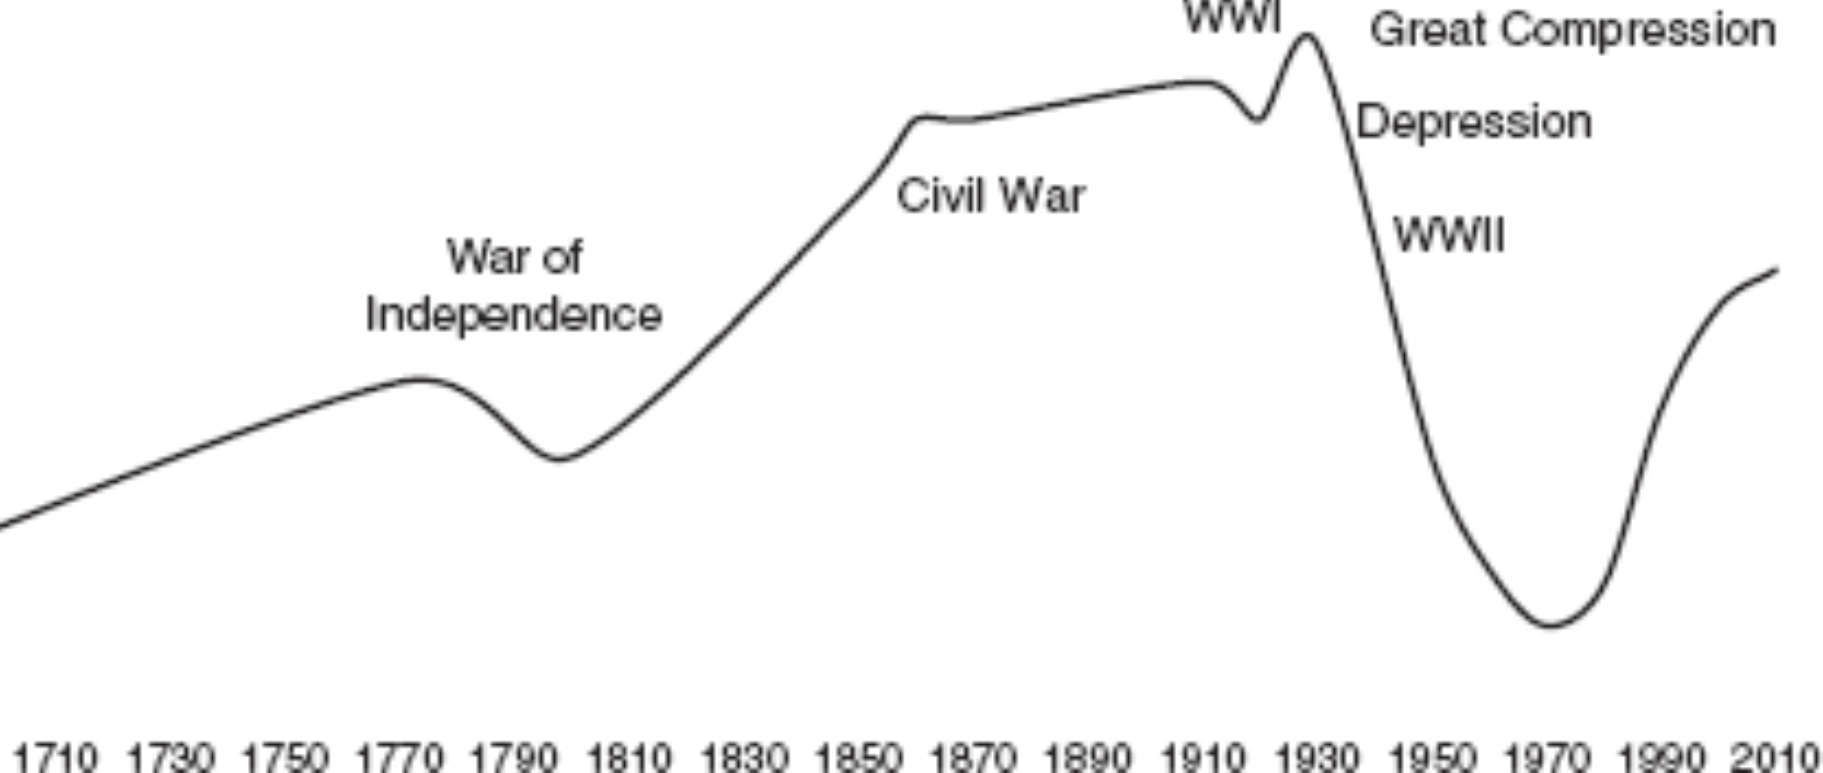
\includegraphics[width = \textwidth]{img/ineq-us}\\\vspace{15pt}United States

\end{frame}
% ----------------------------------------------------

% ----------------------------------------------------
\begin{frame}
\frametitle{Social and institutional legacies}
\centering

\begin{itemize}
  \item How do wars impact macro-level sociopolitical institutions?
  \item Probably the most important thing and what we know less about
\end{itemize}

\end{frame}
% ----------------------------------------------------

% ----------------------------------------------------
\begin{frame}
\frametitle{Social and institutional legacies}
\centering

\begin{itemize}[<+->]
  \item War and state development in medieval Europe, but does that apply to civil war?
  \item Unclear, in many cases, a weak state is the product of civil wars
  \item But for example, the case of {\color{red}{Uganda}}: Museveni established local councils during the civil war, which were later scaled up in the post-war period
\end{itemize}

\end{frame}
% ----------------------------------------------------

% ----------------------------------------------------
\imageframe{img/uganda-pike}
% ----------------------------------------------------

% ----------------------------------------------------
\imageframe{img/state_capacity}
% ----------------------------------------------------

% ----------------------------------------------------
\begin{frame}
\frametitle{Social and institutional legacies}
\centering

\begin{itemize}[<+->]
  \item What should we look at?
  \item[1.] Conflict-wide consequences
  \begin{itemize}
    \item Trying to understand how conflicts in general affect postwar politics
    \item Do conflicts polarize societies? What are the consequences of differente outcomes? etc
    \item E.g. military victory seems to lead to stronger postwar states
  \end{itemize}
\end{itemize}

\end{frame}
% ----------------------------------------------------

% ----------------------------------------------------
\begin{frame}
\frametitle{Social and institutional legacies}
\centering

\begin{itemize}[<+->]
  \item[2.] Micro-level consequences
  \begin{itemize}
    \item Influence of the focus on the micro-dynamics of conflicts
    \item Local- or region-level legacies of wars: how do wars develop at the local level? Wartime institutions, rebel governance?
    \item Legacies of violence: do specific events have consequences?
  \end{itemize}
\end{itemize}

\end{frame}
% ----------------------------------------------------

% ----------------------------------------------------
\begin{frame}
\frametitle{Social processes of civil wars}
\centering

\begin{itemize}[<+->]
  \item Civil wars not only involve changes at the higher power levels, but fundamentally change social and political dynamics at the local level
  \item Directly related to {\color{red}{civilians}}
  \item Changes in local actors, practices, institutions, etc often have long-term consequences in the postwar period, for example:
  \item[1.] Political mobilization
  \item[2.] Polarization of identities
  \item[3.] Gender roles
  % \item[4.] Militarization of local authorities
\end{itemize}

\end{frame}
% ----------------------------------------------------

% ----------------------------------------------------
\begin{frame}
\frametitle{Social processes of civil wars}
\centering

\begin{itemize}[<+->]
  \item[1.] {\color{red}{Political mobilization}}
  \item Prewar mobilization, social movements, wartime mobilization and recruitment, etc
  \item Civilians get much more involved in politics during wars, not only in terms of recruitment, but also in other forms of collective action, offering non-military support, etc
  \item Mobilization varies a lot and depends on armed groups (collaboration networks vs coercion or forced recruitment, etc), wartime events (e.g. reaction to civilian victimization), civilian social structures, etc
\end{itemize}

\end{frame}
% ----------------------------------------------------

% ----------------------------------------------------
\begin{frame}
\frametitle{Social processes of civil wars}
\centering

\begin{minipage}{0.49\textwidth}\centering
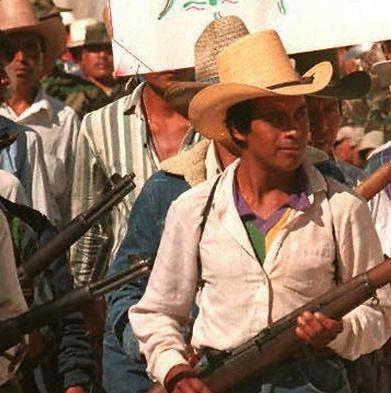
\includegraphics[width = \textwidth]{img/pac}\\
Patrullas de Autodefensa Civil (Guatemala)
\end{minipage}\hfill
\begin{minipage}{0.49\textwidth}\centering
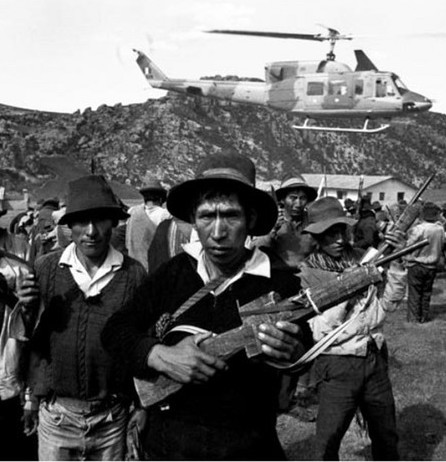
\includegraphics[width = \textwidth]{img/ronda-campesina}\\
Rondas campesinas (Peru)
\end{minipage}

\end{frame}
% ----------------------------------------------------

% ----------------------------------------------------
\imageframe{img/lynching}
% ----------------------------------------------------

% ----------------------------------------------------
\begin{frame}
\frametitle{Social processes of civil wars}
\centering

\begin{itemize}[<+->]
  \item[2.] {\color{red}{Polarization of identities}}
  \item Role of mobilization, militarization, violence, etc
  \item Remember Kalyvas: local cleavages $\neq$ master divisions, at least at the beginning
  \item But as the war goes on, increased alignment, as people choose sides:
  \begin{itemize}
    \item[a.] Opportunistic choice
    \item[b.] Looking for protection
    \item[c.] Moral outrage
  \end{itemize}
  \item Variation within a single conflict: Getting caught `between two fires'? Is it possible to stay neutral? etc
  % \item Forced displacement \& increased polarization/segregation
\end{itemize}

\end{frame}
% ----------------------------------------------------

% ----------------------------------------------------
\begin{frame}<1-2>[label=gender]
\frametitle{Social processes of civil wars}
\centering

\begin{itemize}[<+->]
  \item[3.] {\color{red}{Gender roles}}
  \item War transforms gender roles, with likely long-term consequences
  \item Women combatants comprised more than a quarter of the insurgent force in many civil wars (Peru, Sri Lanka, ...), which introduces a huge change to their traditional social roles
  \item Also: women from rural, isolated areas becoming interlocutors with the state, looking for detainees, etc
\end{itemize}

\end{frame}
% ----------------------------------------------------

% ----------------------------------------------------
\imageframe{img/wwii_women}
% ----------------------------------------------------

% % ----------------------------------------------------
% \begin{frame}
% \frametitle{Social processes of civil wars}
% \centering
%
% \begin{minipage}{0.4\textwidth}\centering
%   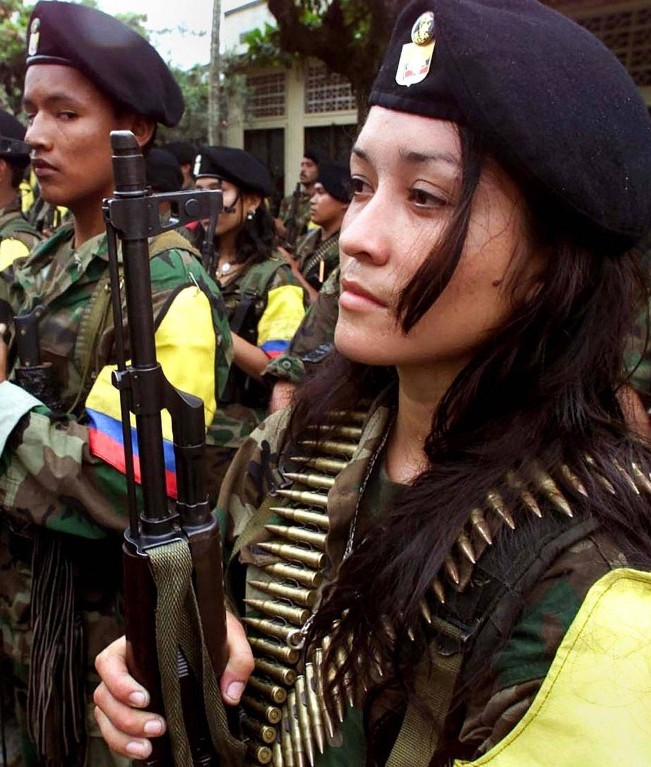
\includegraphics[width = \textwidth]{img/mujeres-farc}\\
%   {\small FARC fighters in Colombia}
% \end{minipage}\hfill
% \begin{minipage}{0.6\textwidth}\centering
%   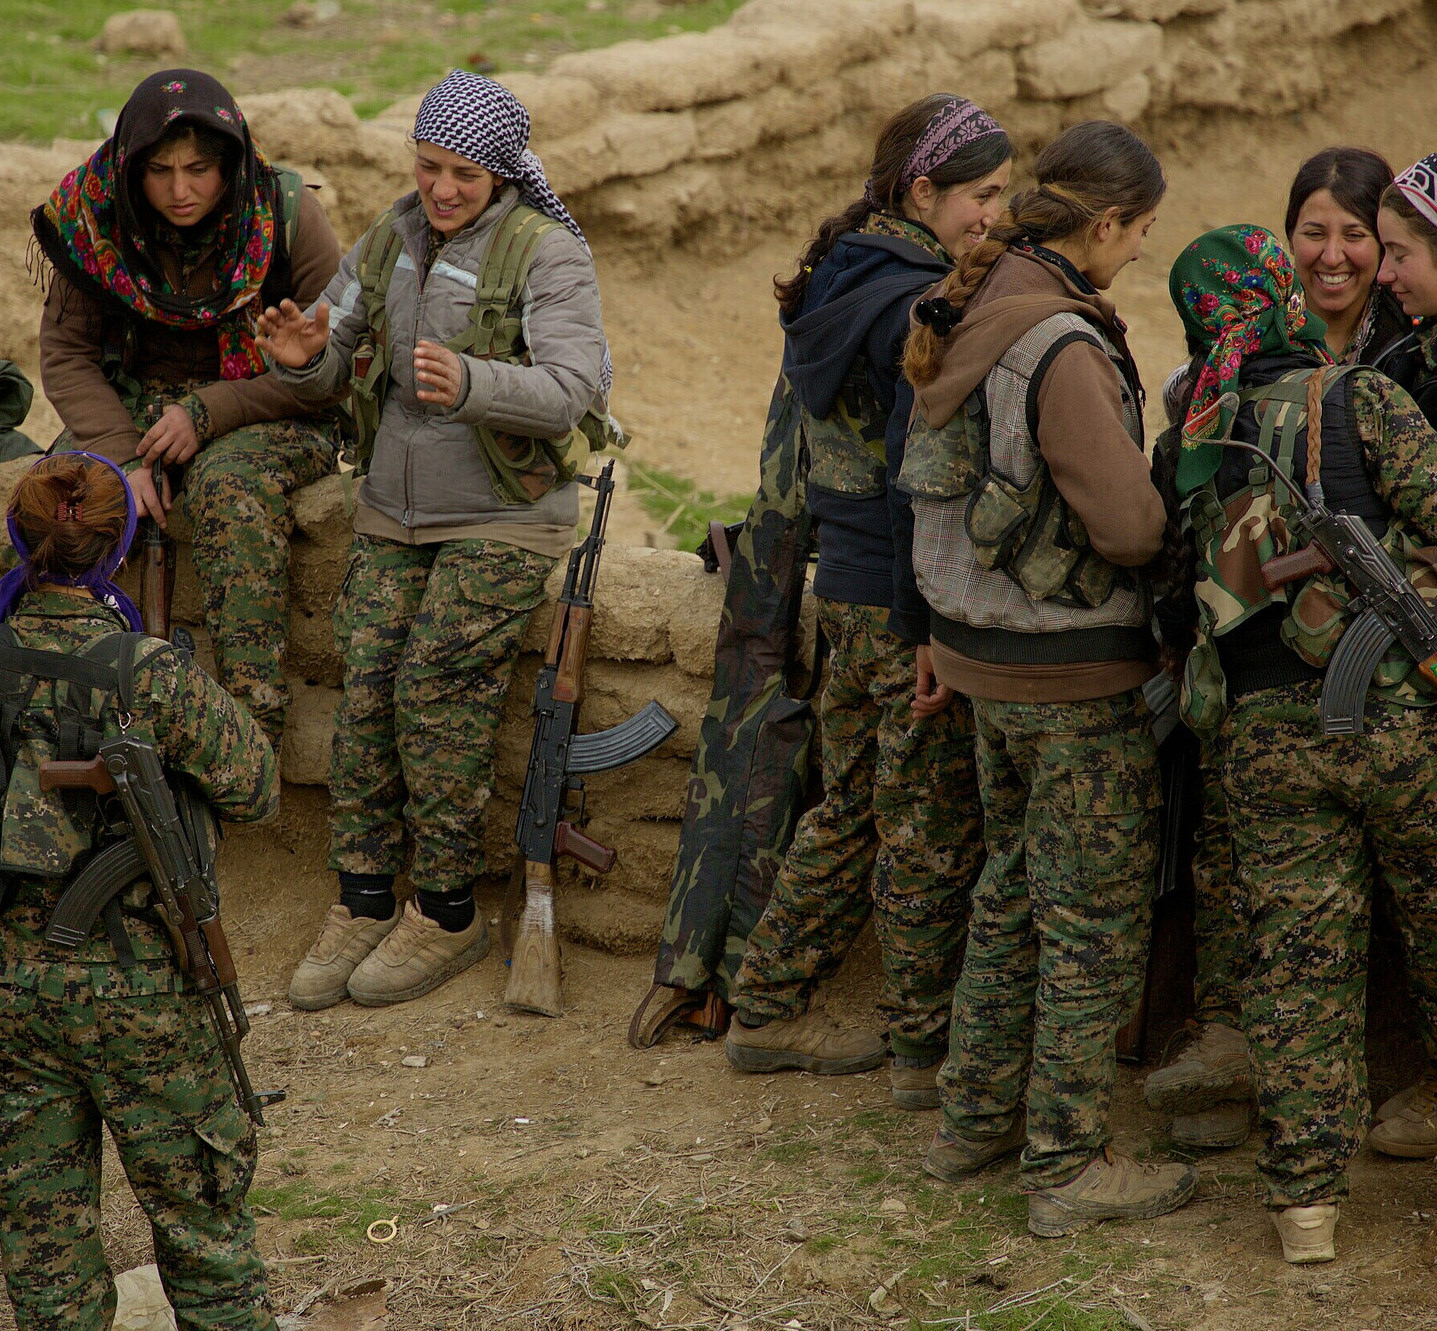
\includegraphics[width = 0.85\textwidth]{img/ypg-women}\\
%   {\small YPG fighters in Rojava, Syria}
% \end{minipage}
%
% \end{frame}
% % ----------------------------------------------------

% ----------------------------------------------------
\imageframe{img/ypg-women}
% ----------------------------------------------------

% ----------------------------------------------------
\againframe<3->{gender}
% ----------------------------------------------------

% ----------------------------------------------------
\imageframe{img/maya_women_guate}
% ----------------------------------------------------

% ----------------------------------------------------
\imageframe{img/plaza_mayo}
% ----------------------------------------------------

% ----------------------------------------------------
\begin{frame}
\frametitle{The legacies of violence}
\centering

\begin{itemize}
  \item What are the long-term consequences of specific events of violence?
\end{itemize}

\end{frame}
% ----------------------------------------------------

% ----------------------------------------------------
\imageframe{img/gernika}
% ----------------------------------------------------

% ----------------------------------------------------
\imageframe{img/gernika_bombing}
% ----------------------------------------------------

% ----------------------------------------------------
\imageframe{img/eta_disarm}
% ----------------------------------------------------

% ----------------------------------------------------
\begin{frame}
\frametitle{Long-term consequences of violence}
\centering

\begin{itemize}[<+->]
\item Do specific events of violence matter?
\item Or is it about discourses and conflict-wide effects?
  \begin{itemize}
    \item If my relative, friend, neighbor was killed, would that change the way I think politically?
  \end{itemize}
\item A lot of this depends on what we think about {\color{red}{how wartime violence happens}} and {\color{red}{whether what happens in a war leaves legacies}}
\end{itemize}

\end{frame}
% ----------------------------------------------------

% ----------------------------------------------------
\begin{frame}
\frametitle{Thinking about legacies of wars}
\centering

\begin{tikzpicture}[every text node part/.style={align=center}]

% square
\draw[-] (-3, 2.5) -- (3, 2.5) node[] {};
\draw[-] (3, 2.5) -- (3, -2.5) node[] {};
\draw[-] (3, -2.5) -- (-3, -2.5) node[] {};
\draw[-] (-3, 2.5) -- (-3, -2.5) node[] {};

% labels
\node (x) at (0, 3.75) {Wartime attitudes?};
\node (x2) at (-1.5, 2.95) [] {Pre-determined};
\node (x3) at (1.5, 2.9) {Endogenous};

\node (y) at (-4.5, 0) {Does wartime\\behavior prevails?};
\node (y) at (-3.6, -1.5) {No};
\node (y) at (-3.6, 1.5) {Yes};

% text
\uncover<2->{\node (a) at (-1.5, 1.5) {Hardening\\thesis};}
\uncover<3->{\node (b) at (1.5, 1.5) {`Photo-finish'\\model};}
\uncover<4->{\node (c) at (-1.4, -1.5) {Civil wars are\\irrelevant};}
\uncover<5->{\node (d) at (1.65, -1.5) {`Wicked\\games'};}

\end{tikzpicture}

\end{frame}
% ----------------------------------------------------

% ----------------------------------------------------
\begin{frame}
\frametitle{Long-term consequences of violence}
\centering

\begin{itemize}[<+->]
  \item The thing is violence {\color{red}{does}} have an effect, and it lasts
  \item How to measure this?
\end{itemize}

\end{frame}
% ----------------------------------------------------

% ----------------------------------------------------
\begin{frame}
\frametitle{Long-term consequences of violence}
\centering

\begin{itemize}[<+->]
  \item If we do focus on how violence affects people's preferences in the long time, what usually happens is a {\color{red}{backfiring effect}}
  \item Old idea: ``The seed of revolution is repression'' (W. Wilson)
  \item But does this happen all the time?
\end{itemize}

\end{frame}
% ----------------------------------------------------

% ----------------------------------------------------
\begin{frame}
\frametitle{Long-term consequences of violence}
\centering

{\small The family had come to accept their secret, and silence helped them to reconcile their experiences with their present reality. They did not dream of revenge [...], neither did they did dream of freedom. {\color{red} They even thought that Franco was a good man who knew nothing of the crimes, injustices, and miseries committed against people like themselves.} When Franco came to Almeria, they went to cheer him.}

{\scriptsize (Account of a victimized family in Almeria, 1957. Cazorla-Sánchez 2009, 3)}\\

\end{frame}
% ----------------------------------------------------

% ----------------------------------------------------
\imageframe{img/villamil_violence}
% ----------------------------------------------------

% ----------------------------------------------------
\imageframe{img/villamil_TOP}
% ----------------------------------------------------

% ----------------------------------------------------
\imageframe{img/did_main_estimates}
% ----------------------------------------------------

% ----------------------------------------------------
\begin{frame}
\frametitle{Long-term legacies}
\centering

\begin{itemize}
  \item It's not only about the consequences of wartime violence
\end{itemize}

\end{frame}
% ----------------------------------------------------

% ----------------------------------------------------
\imageframe{img/lee}
% ----------------------------------------------------

% ----------------------------------------------------
\imageframe{img/prieto}
% ----------------------------------------------------

% ----------------------------------------------------
\imageframe{img/leninopad}
% ----------------------------------------------------

% ----------------------------------------------------
\begin{frame}
\frametitle{The consequences of postwar measures}
\centering

\begin{itemize}
  \item The way these events are \BGyellow{remembered and memorialized} also has consequences, related to effects of TJ policies
  \item Tomorrow's seminar
  \begin{itemize}
    \item {\small \href{https://www.newyorker.com/magazine/2017/12/04/the-fight-over-virginias-confederate-monuments}{The Fight Over Virginia's Confederate Monuments}}
  \end{itemize}
\end{itemize}

\end{frame}
% ----------------------------------------------------


\end{document}
